\section{Multi-Agent Temporal Reconciliation Evaluation}
\label{sec:three-agent-note}

Temporal grounding in QA systems requires not only extracting a date, but reasoning across noisy evidence and model uncertainty.
To isolate this behavior, we built a fully controlled synthetic benchmark where each instance has a known ground-truth year.
The benchmark is designed to test whether multiple models can independently estimate temporal truth and then improve through structured peer revision.

As a focused stress test, we ran a three-agent synthetic benchmark over
120 high-precision questions generated from curated synthetic inputs.
The dataset is split into 60 explicit questions, 20 explicit-multi questions, 20 implicit questions, and 20 multi-implicit questions.
\footnote{Explicit: single timestamp target. Explicit-multi: one sentence mentions two distinct entities, and the target is the release year of the later (latest) entity. Implicit: one non-event claim with a plausible year distribution. Multi-implicit: one sentence combines two implicit claims, with a joint plausible-year distribution.}

Zooming in on the actual protocol, each question is processed in three components.
In \textbf{Initial independent estimates}, three independent models each produce a year prediction and rationale from the same sentence.
In \textbf{Reconciled revisions}, each model revises its answer after seeing the other two predictions and rationales.
In \textbf{Judge synthesis}, a final judge model receives all three revised outputs and produces the final year estimate.
The three agent models are \texttt{gpt-5-mini}, \texttt{gemini-3-flash}, and \texttt{claude-4-5-haiku}.
We intentionally use heterogeneous models to increase viewpoint diversity; this is intended to make reconciliation more informative and improve the value of the final synthesis step.

Scoring is component-specific:
\begin{itemize}
  \item Initial independent estimates accuracy is averaged over all three initial agent predictions for each sample (values are in $\{0,\frac13,\frac23,1\}$), then averaged across samples.
  \item Reconciled revisions applies the same averaging logic over revised predictions.
  \item Judge synthesis is standard binary correctness of the judge output.
\end{itemize}

 This setup avoids an early consensus step and keeps initial independent estimates and reconciled revisions directly interpretable as the strength of cross-model agreement before adjudication.

\begin{figure}[t]
    \centering
    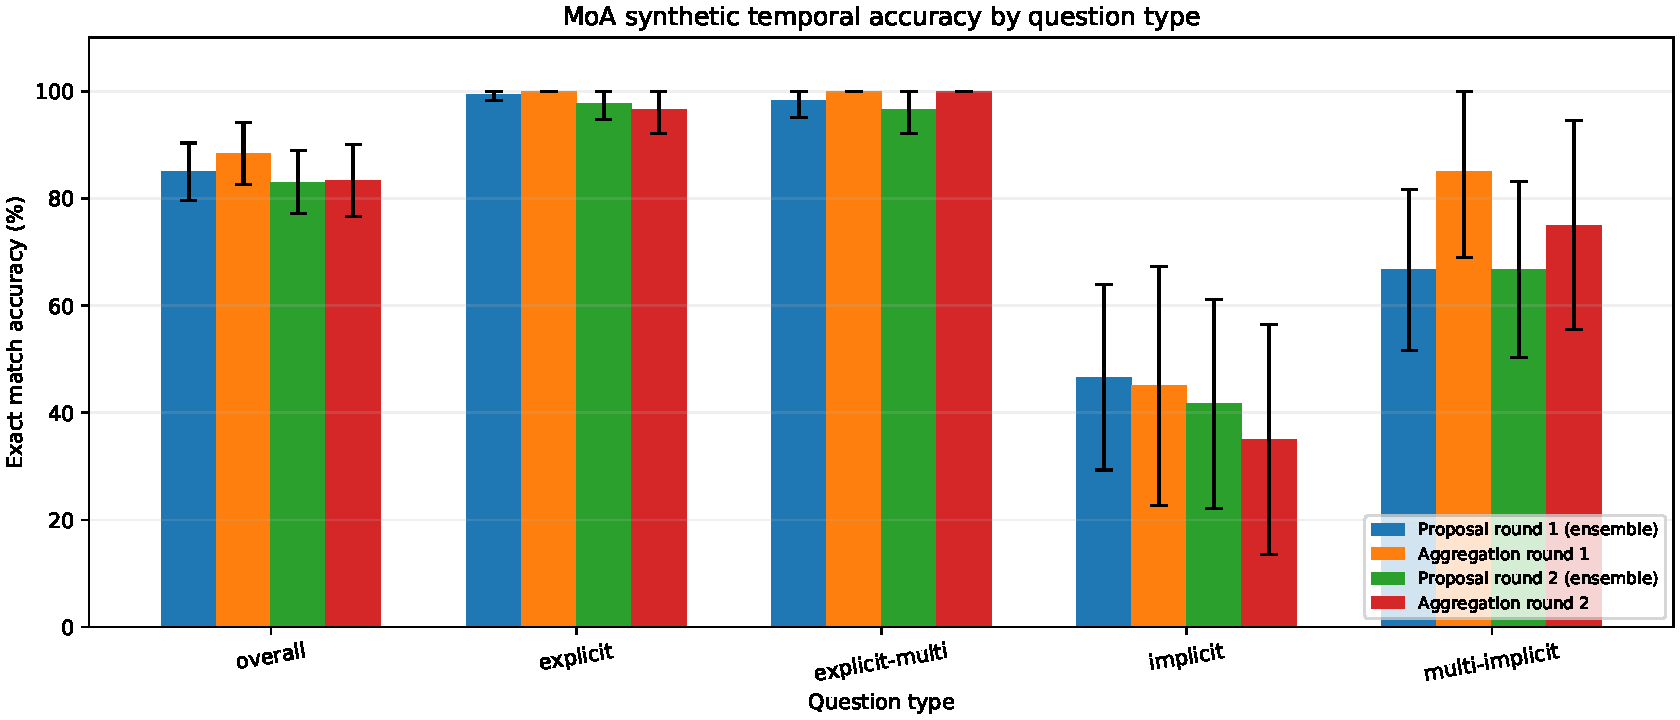
\includegraphics[width=0.88\textwidth]{../data_filtering/synthetic_filtering_eval/results/plots/three_agent_accuracy_by_question_type.pdf}
    \caption{Three-agent synthetic evaluation by question type (explicit, explicit-multi, implicit, multi-implicit) with component-wise exact-match accuracy and 95\% confidence intervals.}
    \label{fig:three-agent-synthetic}
\end{figure}

\begin{figure}[t]
    \centering
    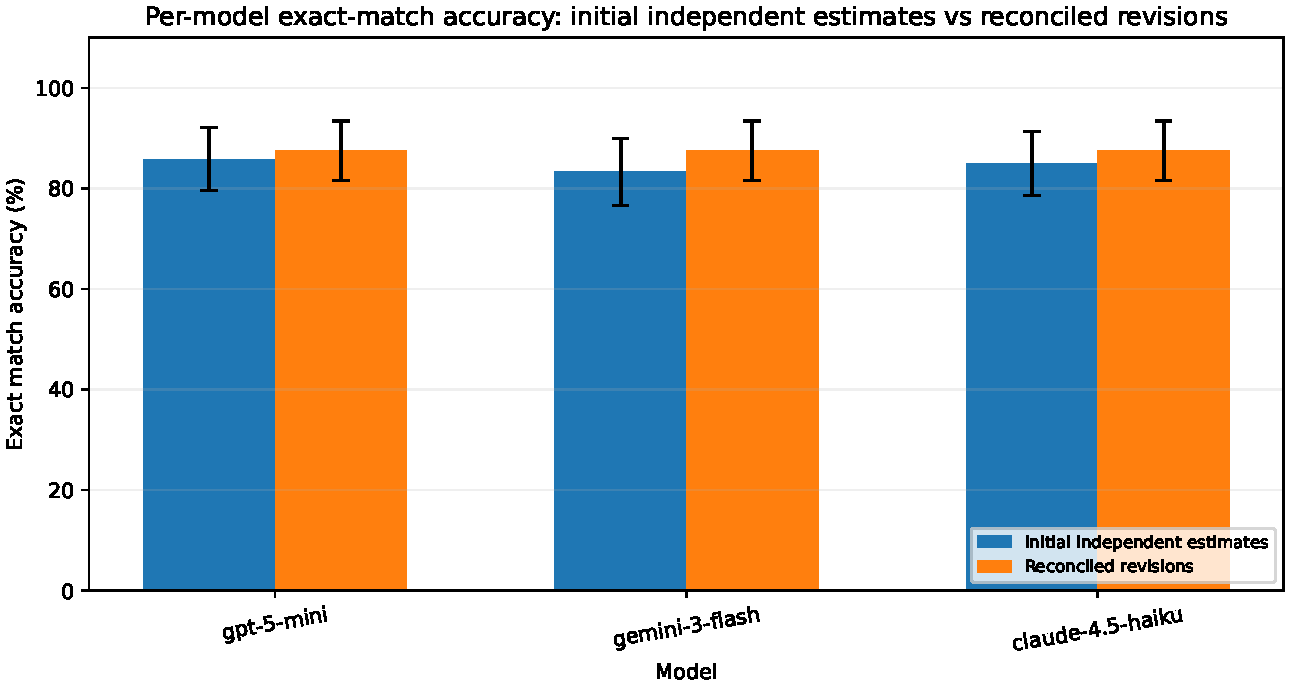
\includegraphics[width=0.88\textwidth]{../data_filtering/synthetic_filtering_eval/results/plots/three_agent_model_pre_post_accuracy.pdf}
    \caption{Per-model exact-match accuracy, comparing initial independent estimates and reconciled revisions.}
    \label{fig:three-agent-per-model}
\end{figure}

Results are summarized in Figure~\ref{fig:three-agent-synthetic} and Figure~\ref{fig:three-agent-per-model}.
We observe near-ceiling performance on explicit settings (explicit and explicit-multi reach 100\% judge accuracy), while implicit settings remain substantially harder (implicit judge accuracy is 50.0\%).
Model-level performance is similar across agents: stage-1 overall exact-match is 85.8\% (gpt-5-mini), 83.3\% (gemini-3-flash), and 85.0\% (claude-4-5-haiku), and all three converge to 87.5\% after reconciled revisions.
The judge setup provides a small net gain overall (84.7\% initial independent estimates $\rightarrow$ 88.3\% judge synthesis), with the clearest improvement on multi-implicit samples.

For implicit samples, we also evaluate distributional alignment using Earth Mover (Wasserstein) distance between each model output distribution (or fallback point mass at the predicted year) and the ground-truth point mass at the true year. We report median distance (lower is better).
\begin{table}[t]
    \centering
    \caption{Implicit-only Wasserstein distance by pipeline component.}
    \label{tab:implicit-wasserstein}
    \begin{tabular}{lcc}
        \hline
        Pipeline component & Median distance (years) & Count \\
        \hline
        Initial independent estimates & 2.492 & 20 \\
        Reconciled revisions & 1.632 & 20 \\
        Judge synthesis & 1.550 & 20 \\
        \hline
    \end{tabular}
\end{table}

\begin{table}[t]
    \centering
    \caption{Multi-implicit Wasserstein distance by pipeline component.}
    \label{tab:multi-implicit-wasserstein}
    \begin{tabular}{lcc}
        \hline
        Pipeline component & Median distance (years) & Count \\
        \hline
        Initial independent estimates & 1.108 & 20 \\
        Reconciled revisions & 0.875 & 20 \\
        Judge synthesis & 0.900 & 20 \\
        \hline
    \end{tabular}
\end{table}

\subsection*{Representative cases}
\label{sec:three-agent-examples}
Table~\ref{tab:three-agent-explicit-example} shows an explicit sample, Table~\ref{tab:three-agent-explicit-multi-example} shows an explicit-multi sample, Table~\ref{tab:three-agent-implicit-example} shows an implicit sample with distributional outputs, and Table~\ref{tab:three-agent-multi-implicit-example} shows a multi-implicit sample.
Table~\ref{tab:three-agent-implicit-initial-all-models} isolates initial independent estimates for the same implicit sentence across all three agent models.
\setlength{\tabcolsep}{3pt}
\renewcommand{\arraystretch}{1.10}
\begin{table}[t]
  \scriptsize
  \centering
  \caption{Explicit sample (id 87), using gpt-5-mini for initial independent estimates and reconciled revisions.}
  \label{tab:three-agent-explicit-example}
  \begin{tabular}{|p{0.16\textwidth}|p{0.76\textwidth}|}
    \hline
    Row label & Text \\
    \hline
    Gold &
    1984 \\
    \hline
    Input &
    ``Leonard Bosack and Sandy Lerner founded Cisco Systems while working at Stanford University.'' \\
    \hline
    Initial independent estimate (gpt-5-mini) &
    ``Leonard Bosack and Sandy Lerner co-founded Cisco Systems while at Stanford in 1984 (company founded in December 1984), so the most likely year associated with this statement is 1984. Final year: 1984.'' \\
    \hline
    Reconciled revision (gpt-5-mini) &
    ``Multiple independent sources (and two other agents) identify 1984 as the founding year; Cisco was founded by Leonard Bosack and Sandy Lerner in December 1984 while at Stanford. The 2001 suggestion refers to a possible publication date, not the historical event. Final year: 1984.'' \\
    \hline
    Judge synthesis &
    ``Cisco Systems was officially incorporated in December 1984 by Leonard Bosack and Sandy Lerner while they were working at Stanford University. Final year: 1984.'' \\
    \hline
  \end{tabular}
\end{table}

\begin{table}[t]
  \scriptsize
  \centering
  \caption{Explicit-multi sample (id 50), using gpt-5-mini for initial independent estimates and reconciled revisions.}
  \label{tab:three-agent-explicit-multi-example}
  \begin{tabular}{|p{0.16\textwidth}|p{0.76\textwidth}|}
    \hline
    Row label & Text \\
    \hline
    Gold &
    2005 \\
    \hline
    Input &
    ``The social networking platform Facebook had been active for about a year by the time YouTube was founded.'' \\
    \hline
    Initial independent estimate (gpt-5-mini) &
    ``Facebook launched in 2004 and YouTube was founded in 2005. The sentence states Facebook had been active about a year by the time YouTube was founded, so the later (latest) year referenced is 2005. Final year: 2005.'' \\
    \hline
    Reconciled revision (gpt-5-mini) &
    ``Facebook launched in 2004 and YouTube was founded in 2005. The sentence compares those two facts and asks for the later year; the later (latest) year is 2005. Final year: 2005.'' \\
    \hline
    Judge synthesis &
    ``Facebook was launched in 2004, and YouTube was founded in 2005. Following the explicit\_multi logic, the target is the later of the two years, which is 2005. Final year: 2005.'' \\
    \hline
  \end{tabular}
\end{table}

\begin{table}[t]
  \scriptsize
  \centering
  \caption{Implicit sample (id 93), using gpt-5-mini for initial independent estimates and reconciled revisions.}
  \label{tab:three-agent-implicit-example}
  \begin{tabular}{|p{0.16\textwidth}|p{0.76\textwidth}|}
    \hline
    Row label & Text \\
    \hline
    Gold &
    ``2015. Gold plausible years: [2015,\allowbreak 2016,\allowbreak 2017,\allowbreak 2018,\allowbreak 2019]. Gold plausible probs: [0.35,\allowbreak 0.30,\allowbreak 0.20,\allowbreak 0.10,\allowbreak 0.05].'' \\
    \hline
    Input &
    ``Adopting carbon-neutral targets is now widely regarded as the essential benchmark for credible climate policy frameworks.'' \\
    \hline
    Initial independent estimate (gpt-5-mini) &
    ``The IPCC Special Report on 1.5C (Oct 2018) explicitly framed reaching net-zero CO2 as necessary to meet 1.5C, which shifted scientific and policy discourse toward carbon-neutral targets. By 2019 (e.g., EU/UK formal adoption of 2050 climate-neutral goals) the view had broadened among major policymakers, so 2018 is the earliest reasonable year with 2019 as the next most plausible. Plausible years: [2018,\allowbreak 2019]. Plausible probs: [0.60,\allowbreak 0.40]. Final year: 2018.'' \\
    \hline
    Reconciled revision (gpt-5-mini) &
    ``Revision after reviewing other agents: the Paris Agreement (Dec 2015) plausibly catalyzed mainstream uptake of carbon-neutral/net-zero as a policy benchmark, so 2015 is now the earliest plausible year. However, the IPCC Special Report on 1.5C (Oct 2018) strongly reframed net-zero as necessary and accelerated policy consensus, so 2018 remains the single most likely year. Major 2019 legislation and pledges (e.g., UK, EU) make 2019 next most plausible. Plausible years: [2015,\allowbreak 2018,\allowbreak 2019]. Plausible probs: [0.30,\allowbreak 0.50,\allowbreak 0.20]. Final year: 2015.'' \\
    \hline
    Judge synthesis &
    ``The 2015 Paris Agreement introduced balancing emissions and removals as an international goal and acted as an early catalyst. The 2018 IPCC report then established net-zero targets as essential for credible climate policy, and this consensus matured in 2019 as major jurisdictions codified these targets. Plausible years: [2015,\allowbreak 2018,\allowbreak 2019]. Plausible probs: [0.25,\allowbreak 0.45,\allowbreak 0.30]. Final year: 2015.'' \\
    \hline
  \end{tabular}
\end{table}

\begin{table}[t]
  \scriptsize
  \centering
  \caption{Multi-implicit sample (id 117), using gpt-5-mini for initial independent estimates and reconciled revisions.}
  \label{tab:three-agent-multi-implicit-example}
  \begin{tabular}{|p{0.16\textwidth}|p{0.76\textwidth}|}
    \hline
    Row label & Text \\
    \hline
    Gold &
    ``2022. Gold plausible years: [2022,\allowbreak 2023,\allowbreak 2024,\allowbreak 2025]. Gold plausible probs: [0.30,\allowbreak 0.40,\allowbreak 0.20,\allowbreak 0.10].'' \\
    \hline
    Input &
    ``Generative AI chatbots are now widely used to summarize the decades of medical consensus regarding the severe health risks associated with cigarette smoking.'' \\
    \hline
    Initial independent estimate (gpt-5-mini) &
    ``Generative-AI chatbots (notably ChatGPT launched Nov 2022) saw explosive uptake, but the characterization 'now widely used' is most defensible beginning in 2023 when multiple LLM chatbots gained broad public and professional use. The medical consensus on smoking's severe health risks has existed for decades prior, so the limiting factor is widespread use of generative chatbots, which became clear in 2023. Plausible years: [2023,\allowbreak 2024]. Plausible probs: [0.85,\allowbreak 0.15]. Final year: 2023.'' \\
    \hline
    Reconciled revision (gpt-5-mini) &
    ``After seeing other agents, I acknowledge late 2022 (ChatGPT public release in Nov 2022) as a plausible earliest date when some users could already be using generative chatbots to summarize medical consensus. However, the phrase 'now widely used' better fits broad public and professional uptake that became clear in 2023. Therefore my point estimate remains 2023 but I assign nontrivial probability (30\%) to late-2022 plausibility and 70\% to 2023. Plausible years: [2022,\allowbreak 2023]. Plausible probs: [0.30,\allowbreak 0.70]. Final year: 2023.'' \\
    \hline
    Judge synthesis &
    ``The claim is temporally anchored by the public availability of generative AI chatbots. While the medical consensus on smoking risks is decades old, the tools to summarize it in this specific manner emerged with the release of ChatGPT in late November 2022. While 2022 is the earliest year the claim could be made, 2023 represents the period when usage became truly 'widespread' across the general public and professional sectors, as indicated by the high probability assigned to that year by all agents. Plausible years: [2022,\allowbreak 2023,\allowbreak 2024]. Plausible probs: [0.20,\allowbreak 0.75,\allowbreak 0.05]. Final year: 2022.'' \\
    \hline
  \end{tabular}
\end{table}

\begin{table}[t]
  \scriptsize
  \centering
  \caption{Implicit sample (id 93): initial independent estimates across all three models.}
  \label{tab:three-agent-implicit-initial-all-models}
  \begin{tabular}{|p{0.16\textwidth}|p{0.76\textwidth}|}
    \hline
    Row label & Text \\
    \hline
    Initial text &
    ``Adopting carbon-neutral targets is now widely regarded as the essential benchmark for credible climate policy frameworks.'' \\
    \hline
    Initial independent estimate (gpt-5-mini) &
    ``The IPCC Special Report on 1.5C (Oct 2018) explicitly framed reaching net-zero CO2 as necessary to meet 1.5C, which shifted scientific and policy discourse toward carbon-neutral targets. By 2019, the view had broadened among major policymakers. Plausible years: [2018,\allowbreak 2019]. Plausible probs: [0.60,\allowbreak 0.40]. Final year: 2018.'' \\
    \hline
    Initial independent estimate (gemini-3-flash) &
    ``The concept of carbon-neutral targets as a primary benchmark for climate policy credibility gained momentum after the late-2018 IPCC 1.5C report. In 2019, countries such as the UK and France legislated these targets, making them standard credibility markers. Plausible years: [2019,\allowbreak 2020,\allowbreak 2021]. Plausible probs: [0.40,\allowbreak 0.40,\allowbreak 0.20]. Final year: 2019.'' \\
    \hline
    Initial independent estimate (claude-4-5-haiku) &
    ``Carbon-neutral targets became widely regarded as essential benchmarks after the Paris Agreement (Dec 2015), which catalyzed mainstream adoption of net-zero commitments. The phrase `now widely regarded' supports the earliest consensus shift around 2015--2016. Plausible years: [2015,\allowbreak 2016,\allowbreak 2017]. Plausible probs: [0.50,\allowbreak 0.30,\allowbreak 0.20]. Final year: 2015.'' \\
    \hline
  \end{tabular}
\end{table}

\section{Related Work}
Our protocol is closest to layered ensemble methods where independent agent outputs are exposed to peers before a final synthesis stage. This mirrors Mixture-of-Agents style pipelines that use parallel first-pass generations and later consolidation layers \cite{wang2025mixtureofagents}. For tasks with a single correct label (such as exact year in explicit settings), self-consistency and voting remain strong baselines and are important controls for whether reconciliation is adding value beyond simple aggregation \cite{wang2022selfconsistency,wang2025ranked}.

The final judge stage is aligned with the LLM-as-a-judge line of work \cite{zheng2023judging,gu2024llmasajudge}. However, judge reliability is a known concern, and judge-centric pipelines can inherit model biases or calibration failures \cite{tan2025judgebench}. This is relevant to our findings where reconciliation does not uniformly improve accuracy across question types.

The reconciliation step itself is related to critique-and-refine and debate-style interaction \cite{madaan2023selfrefine,du2023multiagentdebate}. Prior work also warns that refinement can hurt when critiques are noisy or verification is weak \cite{valmeekam2023selfcritiqueplans}, which is consistent with our motivation for distribution-aware implicit evaluation (Wasserstein) in addition to exact match.

\section{Next Steps}
\begin{enumerate}
  \item Implement the reconciliation stage using the debate-style prompting strategy from \emph{Improving Factuality and Reasoning in Language Models through Multiagent Debate} \cite{du2023multiagentdebate}, and evaluate whether this improves post-revision accuracy and judge-stage outcomes in our synthetic temporal grounding setup.
\end{enumerate}

\bibliographystyle{plain}
\bibliography{../data_filtering/synthetic_filtering_eval/note/related_work}
